\documentclass{article}

\usepackage{amsmath,amssymb}
% \usepackage{fullpage}
\usepackage{enumerate}
\usepackage[hidelinks]{hyperref}
\usepackage{graphicx}
\usepackage{lmodern}
\graphicspath{{../logos/}}


\begin{document}

\setlength{\tabcolsep}{5pt}
\begin{center} \begin{tabular}{cccc}
	% set heights below to 43pt if fullpage not used
	
\includegraphics[height=43pt]{SAMF_logo.jpg} &
	
\includegraphics[height=43pt]{SAICA_logo.jpg} &
	
\includegraphics[height=43pt]{OM_Logo_Stacked_Vignette_on_White_RGB.jpg} &
	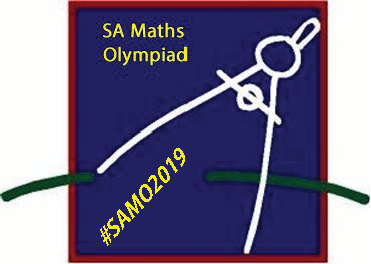
\includegraphics[height=43pt]{SAMO2019.png}
\end{tabular} \end{center}


\bigskip


\begin{center}
\textbf{\Large Senior Monthly Problem Set}
\\ \bigskip
\textbf{\large Due: 4 March 2020}
\end{center}

\begin{enumerate}

\medskip
\item % Malwande, G
Let $ABC$ be a triangle with orthocentre $H$, such that $AB<BC$ and $\angle BAC < 90^\circ$. Let the circle $\Gamma$ centred at $B$ and passing through $A$ intersect $AC$ again at $D$. The circumcircle of $\triangle BCD$ intersects $\Gamma$ again at $E$. $ED$ and $BH$ intersect at $F$. Prove that $BD$ is tangent to the circumcircle of $\triangle DHF$.


\medskip
\item  %IMO Long List 1992 Q65, A
For any 4 points in $\mathbb{R}^3$, does there exist a plane such that the orthogonal projections of the points on the plane make up the vertices of a parallelogram?


\medskip
\item % IMO Long List 1992 Q75, N
Find all positive integers $n$ that can be written in the form:
$$n = \left\lfloor m + \sqrt{m} + \frac{1}{2} \right\rfloor$$
where $m$ is also a positive integer.


\medskip
\item % A Russian Olympiad 1975, C
An $8 \times 8$ chessboard is divided into several regions by 13 straight lines. Can the lines be placed in such a way that each region contains at most 1 centre of the original 64 squares?


\medskip
\item % Adapted from Sharygin 2005, G11 P1, G
Let the midpoints of the sides $BC$, $CA$, $AB$ of an equilateral triangle $ABC$ be $D$, $E$, and $F$ respectively. Let $j$, $k$, and $\ell$ be lines passing through $D$, $E$, and $F$ respectively such that $j \parallel k \parallel \ell$. Define points $P$, $Q$, and $R$ by $P = j\cap EF$, $Q = k \cap FD$, and $R = \ell \cap DE$. Prove that the points $X$, $Y$, and $Z$ defined by $X = BC \cap QR$, $Y = CA \cap RP$, and $Z = AB \cap PQ$ are  collinear.


\medskip
\item % Mongolia 2008 TST Day 3 Q3
Show that there are only finitely many solutions $(x, y) \in \mathbb{N}^2$ to the equation
$$\sum_{i = 1}^{m} (x + i)^n = \sum_{i = 1}^{m} (y + i)^{2n}$$
where $m, n \in \mathbb{N} \setminus \{1\}$ are given constants.


\medskip
\item % Spain, Round 2, 1992
In the land of Graphopia there are $n$ towns. Between some pairs of towns there are direct roads. The residents of these towns want to have mathematics tournaments. They've decided that in order to have a mathematics tournament they need to have $a$ participating towns. Further they decide that in order to have a tournament the connections between the towns involved must be symmetrical. That is either every pair of towns in a tournament are directly linked by a road or no pair is. 

As mathematics competitions are rightly adored by every member of Graphopia every grouping of $a$ towns that can hold a tournament holds one once a year (some towns may be in multiple groupings). However in some years new roads are built and old ones lost to the elements. If a group of $a$ towns find themselves able to put on a tournament they immediately do. If a tournament finds itself unallowable due to road connections, that tournament is regretfully discontinued. Prove that it is possible that one year poor Graphopia finds itself having less than $\binom{n}{a} $$2^{1-\binom{a}{2}}$ tournaments.


\medskip
\item % Serbian Mathematical Olympiad 2007
For positive real numbers $a$, $b$, and $c$ with $a+b+c=1$ prove that:
\begin{align*}
 	\frac{a^{n+2}}{a^{n+1} + b^n + c^n} + \frac{b^{n+2}}{a^n + b^{n+1} + c^n} + \frac{c^{n+2}}{a^n + b^n + c^{n+1}} \ge \frac{1}{7}
\end{align*}

where $n \in \mathbb{N}$. Where does equality occur?

\end{enumerate}


\vfill
\textbf{\Large Email submission guidelines}
\begin{itemize}
	\item Email your solutions to \href{mailto:samf.training.assignments@gmail.com}{\texttt{samf.training.assignments@gmail.com}}.
	\item In the subject of your email, include your name and the level of the assignment (Beginner, Intermediate or Senior).
	\item Submit each question in a single separate PDF file (with multiple pages if necessary), with your name and the question number written on each page.
	\item If you take photographs of your work, use a document scanner such as Office Lens to convert to PDF.
	\item If you have multiple PDF files for a question, combine them using software such as PDFsam.
\end{itemize}

\end{document}